\documentclass[12pt]{pom_thesis}

\usepackage[]{algorithm2e}
\usepackage{tikz}
\usepackage{ifthen}
% This first part of the file is called the PREAMBLE. It includes
% customizations and command definitions. The preamble is everything
% between \documentclass and \begin{document}.
\usepackage{amsthm}
\newtheorem{theorem}{Theorem}
\usepackage[margin=1in]{geometry}  % set the margins to 1in on all sides
\usepackage{graphicx}              % to include figures
\usepackage{amsmath}               % great math stuff
\usepackage{amsfonts}              % for blackboard bold, etc
\usepackage{amsthm}                % better theorem environments
\usepackage{changepage}
\usepackage{lipsum}                     % Dummytext
\usepackage{xargs}                      % Use more than one optional parameter in a new commands
 % Coloured text etc.
% 
\usepackage[colorinlistoftodos,prependcaption,textsize=tiny]{todonotes}
\newcommandx{\unsure}[2][1=]{\todo[linecolor=red,backgroundcolor=red!25,bordercolor=red,#1]{#2}}
\newcommandx{\change}[2][1=]{\todo[linecolor=blue,backgroundcolor=blue!25,bordercolor=blue,#1]{#2}}
\newcommandx{\info}[2][1=]{\todo[linecolor=OliveGreen,backgroundcolor=OliveGreen!25,bordercolor=OliveGreen,#1]{#2}}
\newcommandx{\improvement}[2][1=]{\todo[linecolor=Plum,backgroundcolor=Plum!25,bordercolor=Plum,#1]{#2}}
\newcommandx{\thiswillnotshow}[2][1=]{\todo[disable,#1]{#2}}
\newcommand{\blockmatrix}[9]{
	\draw[draw=#4,fill=#5] (0,0) rectangle( #1,#2);
	\ifthenelse{\equal{#6}{true}}
	{
		\draw[draw=#7,fill=#8] (0,#2) -- (#9,#2) -- ( #1,#9) -- ( #1,0) -- ( #1 - #9,0) -- (0,#2 -#9) -- cycle;
	}
	{}
	\draw ( #1/2, #2/2) node { #3};
}

% Quick implementation of a tikz right parenthesis
% \rightparen{width}
\newcommand{\rightparen}[1]{
	\begin{tikzpicture} 
	\draw (0,#1/2) arc (0:30:#1);
	\draw (0,#1/2) arc (0:-30:#1);
	\end{tikzpicture}%this comment is necessary
}

% Quick implementation of a tikz left parenthesis
% \leftparen{width}
\newcommand{\leftparen}[1]{
	\begin{tikzpicture} 
	\draw (0,#1/2) arc (180:150:#1);
	\draw (0,#1/2) arc (180:210:#1);
	\end{tikzpicture}%this comment is necessary
}

% Unframed block matrix, "m" prefix to match fbox, mbox
% \blockmatrix[r,g,b]{width}{height}{text}
\newcommand{\mblockmatrix}[4][none]{
	\begin{tikzpicture} 
	\ifthenelse{\equal{#1}{none}}
	{
		\blockmatrix{#2}{#3}{#4}{none}{none}{false}{none}{none}{0.0}
	}
	{
		\definecolor{fillcolor}{rgb}{#1}
		\blockmatrix{#2}{#3}{#4}{none}{fillcolor}{false}{none}{none}{0.0}
	}
	\end{tikzpicture}%this comment is necessary
}

% Framed block matrix
% \fblockmatrix[r,g,b]{width}{height}{text}
\newcommand{\fblockmatrix}[4][none]{
	\begin{tikzpicture} 
	\ifthenelse{\equal{#1}{none}}
	{
		\blockmatrix{#2}{#3}{#4}{black}{none}{false}{none}{none}{0.0}
	}
	{
		\definecolor{fillcolor}{rgb}{#1}
		\blockmatrix{#2}{#3}{#4}{black}{fillcolor}{false}{none}{none}{0.0}
	}
	\end{tikzpicture}%this comment is necessary
}

% Diagonal block matrix
% \dblockmatrix[r,g,b]{width}{height}{text}
\newcommand{\dblockmatrix}[4][none]{
	\begin{tikzpicture} 
	\ifthenelse{\equal{#1}{none}}
	{
		\blockmatrix{#2}{#3}{#4}{black}{none}{true}{black}{none}{0.35cm}
	}
	{
		\definecolor{fillcolor}{rgb}{#1}
		\blockmatrix{#2}{#3}{#4}{black}{none}{true}{black}{fillcolor}{0.35cm}
	}
	\end{tikzpicture}%this comment is necessary
}


% Diagonal block matrix, but exposes diagonal offset
% \diagonalblockmatrix[r,g,b]{width}{height}{text}
\newcommand{\diagonalblockmatrix}[5][none]{
	\begin{tikzpicture} 
	
	\ifthenelse{\equal{#1}{none}}
	{
		\blockmatrix{#2}{#3}{#4}{black}{none}{true}{black}{none}{#5}
	}
	{
		\definecolor{fillcolor}{rgb}{#1}
		\blockmatrix{#2}{#3}{#4}{black}{none}{true}{black}{fillcolor}{#5}
	}
	
	\end{tikzpicture}%necessary comment
}

\newcommand{\valignbox}[1]{
	\vtop{\null\hbox{#1}}% necessary comment
}

% a hack so that I don't have to worry about the number of columns or
% spaces between columns in the tabular environment
\newenvironment{blockmatrixtabular}
{% necessary comment
	\begin{tabular}{
			@{}l@{}l@{}l@{}l@{}l@{}l@{}l@{}l@{}l@{}l@{}l@{}l@{}l@{}l@{}l@{}l@{}l@{}l@{}l
			@{}l@{}l@{}l@{}l@{}l@{}l@{}l@{}l@{}l@{}l@{}l@{}l@{}l@{}l@{}l@{}l@{}l@{}l@{}l
			@{}l@{}l@{}l@{}l@{}l@{}l@{}l@{}l@{}l@{}l@{}l@{}l@{}l@{}l@{}l@{}l@{}l@{}l@{}l
			@{}
		}
	}
	{
	\end{tabular}%necessary comment
}
% various theorems, numbered by section


\DeclareMathOperator{\id}{id}

\newcommand{\bd}[1]{\mathbf{#1}}  % for bolding symbols
\newcommand{\RR}{\mathbb{R}}      % for Real numbers
\newcommand{\ZZ}{\mathbb{Z}}      % for Integers
\newcommand{\col}[1]{\left[\begin{matrix} #1 \end{matrix} \right]}
\newcommand{\comb}[2]{\binom{#1^2 + #2^2}{#1+#2}}
\usepackage{graphicx}
\usepackage{csquotes}
\usepackage{lipsum}
\newcommand\tab[1][1cm]{\hspace*{#1}}

\begin{document}


\nocite{*}

\title{Data Representation as Low Rank Matrix Factorization}


\author{Ziv Epstein \\ 
	\texttt{ziv.epstein@pomona.edu}}
\advisor{Blake Hunter}
\maketitle
\pagenumbering{arabic}
\tableofcontents
\newpage


\abstract{ 
	A growing body of literature suggests that visual perception and representation is the result of a hierarchical relation network, whereby nodes that contain values on global properties are scaffolded with increasing levels of representational complexity. Here, we explore algorithms that represent data as low-dimensional approximations. 
	}
\begin{chapter}{Introduction}
	There is a growing interest in the computational and mathematical science in the development of algorithms that can automatically create understanding about data corresponding to some phenomenon. As an explosion of data collection and distribution systems have become the mainstream, there is now more data available than humans observers to understand it. Thus the need for automated algorithms that can infer patterns and relationships within data is self evident. 
	
	Here, I will consider the case were data is represented as a well-structured and  real-valued matrix. This approach can represent data from a large range of domains, such as sound, natural language, visual images and networks. Thus, many of the algorithms and heuristics I explore here are domain general, and can be applied with success to a range of settings. 
	
	My particular focus in this thesis is the notion of \textit{low-dimensional representations of data}. A real valued matrix $X$ that represents a collection of sounds, natural language documents, images or networks taken from real world settings will necessarily be noisy and not optimally structured. One canonical challenge (that we will dub ``The Representation Problem'') is to find a $X' \approx X$ that well approximates the original data's structure, but with $\operatorname{rank}(X') << \operatorname{rank}(X)$. A low rank approximation of the data gives a sparse representation that in some sense captures the most important facets of the data. 
	
	This approach also has explanatory power. Let $r = \operatorname{rank}(X')$ and $b= (b_1,b_2,\cdots,b_r)$ be a basis for $X'$. Depending on the constraints imposed on the $b_i$'s, they can have many different interpretations. For example, when the $b_i$'s are constrained to be orthonormal to each other, the resulting algorithm is Principal Component Analysis (PCA), which ``supplies the user with a lower-dimensional projection of the object when viewed from its most informative viewpoint.'' 
	
	Since our mission is to emulate human understanding, a natural starting place for inspiration is the human brain. Indeed there is a long-standing tradition in computer and information science to algorithmically model the information processing systems the brain uses to make sense of the world. However, I hope to also go one step deeper. In addition to an overview of many of the important algorithms used today, we will explore the cognitive implications of these algorithms. In particular, I aim to invert the paradigm of using neural architecture to inform algorithms: I will use algorithms to inform notions of neural architecture. By creating a bilateral dialogue between the cognitive and computer sciences, I hope this work will help to bridge the gaps between the two fields by I) equipping the cognitive ideas of neural information processing with a notational formalism consist with the algorithms research and II) contextualizing the algorithms research whereby it is clear how it might relate to the acquisition of human knowledge.
\end{chapter}

\begin{chapter}{Theories for Human Image Understanding}
	The general class of algorithms I am considering have in the common the fact that they take as input a large amount of noisy, somewhat structured data, and output some unified high-level notion of underlying pattern. 
	\begin{figure}[h]
		\label{cup}
		\centering
		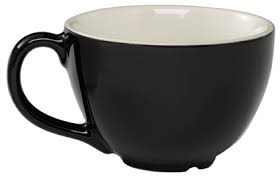
\includegraphics[width=3in]{cup}
		\caption{How does your brain take the raw retinal activations of this picture and produce a mental representation of a cup?}
	\end{figure}
	Thus in many ways they emulate the most successful raw data to high-concept pipeline: the human vision system. When starting at a cup, our brains take  in thousands of raw retinal activities, and through a complex schema of neural information processing, result in a high-level conceptualization of a cup. The intricacies of this pipeline are not fully understood, but many of the driving mechanisms are. To motivate the algorithmic approach, I begin with a short overview of the pervading theories for human image understanding. 

\section{Part-based recognition and visual perception}
A given object can project an uncountable infinitude of possible visual configurations to the human retina. Thus the phenomenon of how raw visual input to the visual system is represented as robust concepts in the human mind has long haunted philosophers, cognitive scientists, mathematicians and computer scientists. Empirical observation imposes several axioms that any repsectable theory of object recognition must take into account, which Biederman enumerates:
\begin{enumerate}
	\item \textbf{Imprecise attention to detail:} ``Access to the mental representation of an object should not be dependent on the absolute judgments of quantitative detail. For example, distinguishing among just several levels of the degree of curvature or length of an object typically requires more time that that retuqired for the identifcation of the object itself.''
	\item \textbf{Topological fuzziness:} ``The information that is the basis for recognition should be relatively invariant with respect to orientation and modest degradation'.'
	\item \textbf{Plasticity:} ``Partial matches should be computable. A theory of object interpretation should have some principled means for computing a match for occluded, partial or new exemplars of a given category.''
\end{enumerate}
These axioms are central to task of modeling, and will be used by the cognitive and mathematical models put forward here. A large number of explanatory theories have been proposed over the years for this phenomenon of object recognition. One extremal idea is the structuralist position which posits that ``the perception of whole figures is nothing more than the concatenation of primitive perceptual elements.'' \cite{palmer1977hierarchical}. Another extremal theory, born out of the Gestalt theory, claims that the recognition of complex objects is an indivisible process, which cannot be reconstructed by considering the nature and properties of its constituent parts.  The most performant modern theories lie within the simplex defined by these holistic and atomic extrema. One such theory, the Recognition-by-Components (RBC) theory proposed by Biederman proposes a sparse vocabulary of atoms and a schema for how these components can be conglomerated to represent in memory (see Figure~\ref{fig: rbc}) \cite{biederman1987recognition}.
\begin{figure}
	\label{fig: rbc}
	\centering
	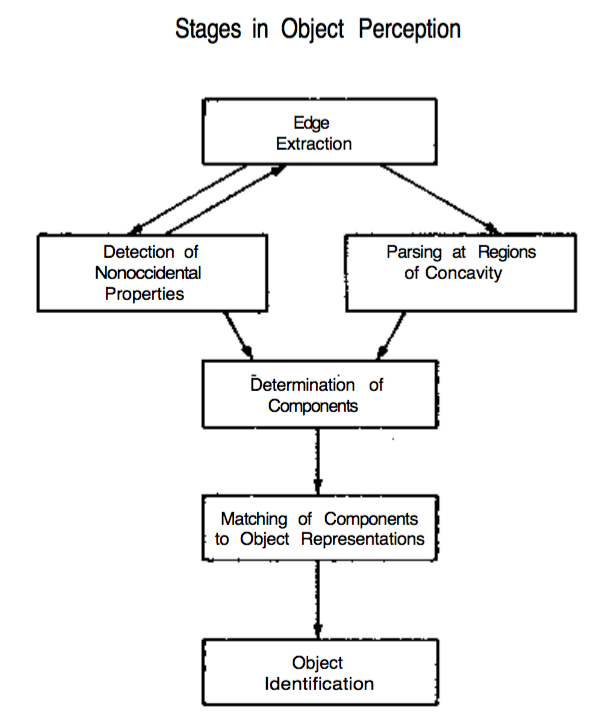
\includegraphics[width=6cm]{rbc}
	\caption{Processing stages for object recognition proposed by the RBC Theory. Adapted from \cite{biederman1987recognition}}
\end{figure}
First, edges are extracted from the raw sensory data received from the optical system. Local properties of the input, such as luminance, texture and color, aid in providing robust edge segmentations. Then, in parallel, the parsing of the concave regions and the identification of nonaccidental properties is performed. The latter provides ``critical constraints on the identity of the components. Then these processes coalesce to form a specific arrangement of components, which are then matched against pre-existing representations in memory. The representation that best ``matches'' the observed arrangement gives rise to the actual object identification. 

Since RBC uniquely relates to the visual system, the components Biederman proposes are a set of generalized cones called \textbf{geons} (for ``geometric ions'') \cite{biederman1987recognition}.
A victory for RBC is its explanatory vastness with a small number of components. Biederman suggests that 36 geons is sufficient to represent all objects that humans can differentiate between. 

RBC has two heuristics that we will primary draw upon for formalizing this theory of object recognition with formal models. The first is this ability to represent the nuance of human perception with a small number of components. In mathematical terms, these components form a linearly independent \textbf{basis}, by which any object, $O$, can be approximated:
\begin{equation} \label{eq:1}O = \sum_{i=1}^d \alpha_i b_i\end{equation}
where $d$ is much smaller than the space of possible objects. Natural questions that arise from this model of human perception are 1) What is sufficient for $d$? Biederman proposes $d=36$ is sufficient of visual object recognition, but what about other domains? and 2) How are these bases, $b_i$ learned? Biederman suggests that $b_i$ is a volumetric cone, but gives no explanation for how this components emerge from the human visual system. 

The second heuristic of RBC we will use the schematic for recognition (see Figure \ref{fig: rbc}). This schema gives us a roadmap for a suite of algorithms we will use to generate representational models (see Section \ref{chapter:techniques}). 
\section{Knowledge representation as information retrieval}
The RBC Theory puts forward a highly structured representation of a given input $O$ as described in Equation \ref{eq:1}. It then suggests that this representation is then procedural matched with a preexisting notion in memory towards recognition. To understand how this matching occurs, we turn to Minsky's framework for representing knowledge \cite{minsky1975framework}. Minsky thinks of memory as a collection of \textbf{frames}, which is a data structure that represents a stereotyped situation, space or object \cite{minsky1975framework}. In particular, a frame is a hierarchical network of nodes and relations which correspond to that which the frame represents. In particular, the ``top levels'' of the network are fixed. They represent entities and relations that are always true about the frame's content. The lower lever has \textbf{terminals}, empty ``slots'' to be filled with raw input or data. These terminals carry with them a set of rules (which are frames themselves) which specify the necessary conditions for assignment that terminal. 

Large collections of these frames are aggregated into structures called \textbf{frame-systems}, where related frames are proximal. In particular, actions in the world correspond to \textbf{transformations} in the frame-system, whereby similar objects have a smooth transformation between them. For example, different frames might correspond to observing a room at different angles, and the transformation between adjacent frames corresponds to the observer moving to change their vantage point \cite{minsky1975framework}. These frame-systems are further connected into a \textbf{information retrieval network}. 

After the raw sensory input of a stimulus percolates through the RBC processing system outlined in Figure 2, it finally reaches a component representation that must be matched with a frame. This process is done as follows. For a given frame $F^i$ with top levels $f^i$ and terminals $t^i$, the features of the representation are assigned to the frame's terminals, $t_i$. In the assignment sufficiently conforms for the specifications of the terminals (i.e. their corresponding frames $F_{t_i}$, and the top level nodes $f_i$), the object is identified as in the last stage of Figure 2.1. However if the proposed frame cannot conform to the terminal specifications, then the information retrieval system repeatedly puts forward another frame until a candidate fits the condition.

This process of selecting an optimal frame for representation is parallel to the optimization component of the algorithms we will discuss.  
\section{The hierarchical structure of perception}
Biederman puts forward an atomic unit of visual perception \cite{biederman1987recognition}, and Minksy extends that notion with a generalized framework for representing this atomic units \cite{minsky1975framework}. However neither of these formulations describe explicitly how raw sensory data can be accumulated into something as sophisticated as the high-level recognition of an object. Palmer puts forward a structural schematic for hierarchical perceptual representation involving structural units, values on global properties and structural relationships (see Figure \ref{fig:palmer}) \cite{palmer1977hierarchical}. 
\begin{figure}[h]
	\label{fig:palmer}
	\centering
	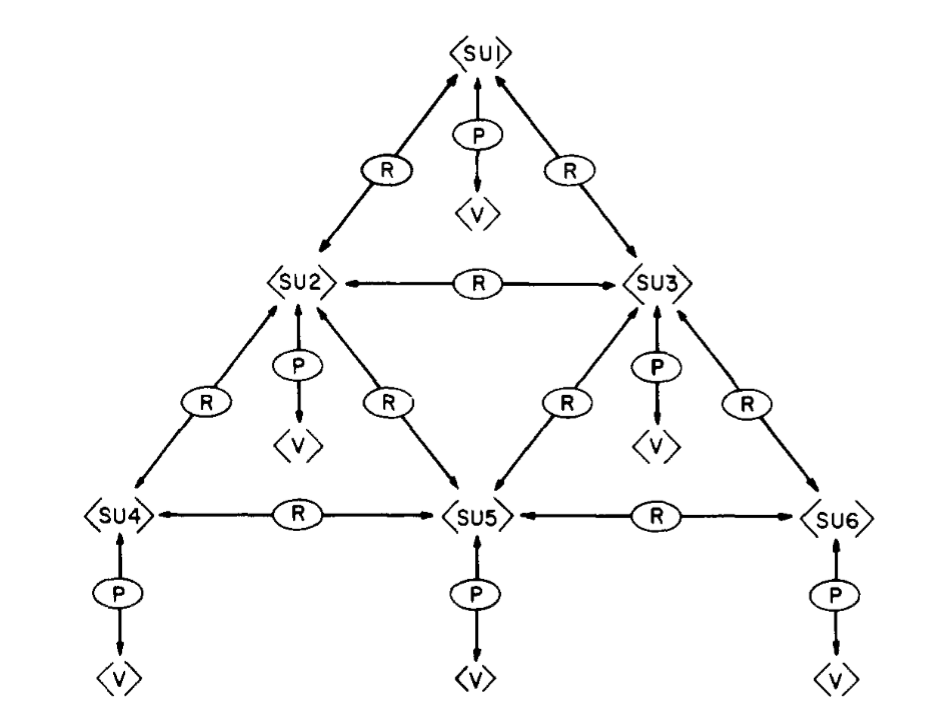
\includegraphics[width=10cm]{palmer_tree}
	\caption{The hierarchical relationship network used to represent perceptual information. At each level of the hierarchy, a structural unit (SU) is a combination of values (V) on global properties (P) and structural relationships to other structural units.  Adapted from \cite{palmer1977hierarchical}}
\end{figure}
The values of the global properties at each node of the network are a real-valued vector ``along perceptual dimensions relative to some referent.'' \cite{palmer1977hierarchical}. During the process of pattern recognition, these numeric values are used to evaluate the goodness-of-fit between some raw sensory input (that is to be identified) and some pre-existing information encoded in the network. The task of matching the sensory input to the encoded information is analogous to Minsk'y frame retrieval discussed above \cite{minsky1975framework}.
\section{Interpretations for Algorithmic Formulation}
\label{interp}
The theories put forward above have several key formulations of the Representation Problem that I will leverage and formalize throughout this thesis. 

\textbf{Object Classification as Supervised Manifold Learning}

As we have seen, the hierarchies proposed above aim to match high-order labels to a series of raw retinal activations. For example, let $(r_1,r_2,\cdots, r_n)$ be the retinal activation of observing Figure \ref{cup}. Previous to observing the image, there exists somewhere in the perceptual hierarchy of your brain the label of cup $\ell_i$. Thus the task of object classification  can be formulated as the supervised learning of a manifold $f$, whereby $f(r_1,r_2,\cdots,r_n) = \ell_i$.

\textbf{Geons as Topics}

\textbf{Hierarchical Organization of Topics}
\todo{finish these and make figures}
\end{chapter}

\begin{chapter}{Techniques}
	\label{chapter:techniques}
\section{Singular Value Decomposition}
The first technique to represent a matrix $X$ is to factorize it using singular value decomposition. 

\begin{theorem}
	Suppose  $X \in \mathbb{R}^{m \times n}$, then there exists a factorization, called the singular value decomposition of $X$, of the form 
	$$X= U \Sigma V^T$$ 
	where $U \in \mathbb{R}^{m \times m}$ is unitary, $\Sigma \in \mathbb{R}^{m \times n}$ with non-negative real numbers on the diagonal and $V^T \in \mathbb{R}^{n \times n}$ is unitary. 
\end{theorem}
The diagonal entries $\sigma_i$ of $\Sigma$ are called the \textbf{singular values} of $X$.

\begin{proof}(Bast) Observe that $X^TX \in \mathbb{R}^{n \times n}$ is symmetric. Thus, there exist $n$ eigenvectors $v_1,\cdots,v_r$ with corresponding eigenvalues $\lambda_1,\cdots,\lambda_r$ that are pairwise orthogonal (i.e. $v^T_iv_j=0 \ \forall i \neq j$) with $r = \text{rank}(X^TX) = \text{rank}(X)$. Furthermore, we have that $X^TX = VDV^T$, where $V=[v_1,\cdots,v_n] \in \mathbb{R}^{n\times n}$ and  $$d = \begin{bmatrix}
	\lambda_1  & 0     & \cdots             & 0    \\
	0  & \lambda_2 & \cdots & 0        \\
	\vdots  & \vdots & \ddots & \vdots &     \\
	0 & 0 & \cdots & \lambda_n
	\end{bmatrix}.$$ 
	Since $v_i$ is an eigenvector for $X^TX$, observe that $XX^TXv_i = X\lambda_iv_i=\lambda_iXv_i$. Which is to say that if  $v_i$ is an eigenvector for $X^TX$, then  $Xv_i$ is an eigenvector for $XX^T$ with the same eigenvalue $\lambda_i$. Now we can compute the squared norm of $XV_i$ as follows
	$$||XV_i||^2 = (Xv_i)^T(Xv_i)=v_i^TX^TXv_i = v_i^T\lambda_i v_i = \lambda_i v_i^T v_i$$
	So the norm of $XV_i = \sqrt{\lambda_i} = \sigma_i.$ Now let $u_i=Xv_i\sigma_i$. Then we have 
	$$u_i^TXv_j = (Xv_i/\sigma_i)^TXv_j = \frac{v_i^TX^TXv_j}{\sigma_i} = v_i^Tv_j \times \frac{\lambda_i}{\sigma_i}$$
	which is to say $u_i^TXv_j=0$ if $i\neq j$ and $u_i^TXv_j=\sigma_i$ if $i=j$. Now writing these equations for $i=1,\cdots,r$ yields
	 $$\begin{bmatrix}
	 u_1^T \\
	 u_2^T        \\
	 \vdots      \\
	 u_r^T 
	 \end{bmatrix} \cdot X \cdot [v_1 \cdots v_r] =  \begin{bmatrix}
	 \sigma_1  & 0     & \cdots             & 0    \\
	 0  & \sigma_2 & \cdots & 0        \\
	 \vdots  & \vdots & \ddots & \vdots &     \\
	 0 & 0 & \cdots & \sigma_r
	 \end{bmatrix}$$
	 Since $u_i \in \mathbb{R}^m$, the lefthand matrix we have is a $r \times m$ matrix. Thus we generate $u_i$ for $i=r+1,\cdots,m$ to expand the matrix to be $m \times m$ by arbitrarily picking unit vectors that are pairwise orthogonal and orthogonal to $u_1,\cdots,u_r$. Similarly for the $v_i$'s, we generate $v_i$ for $i=r+1,\cdots,n$ to expand the matrix to be $n \times n$ by arbitrarily picking unit vectors that are pairwise orthogonal and orthogonal to $v_1,\cdots,v_r$. This extension gives us in matrix form
	 	 $$\begin{bmatrix}
	 	 u_1^T \\
	 	 u_2^T        \\
	 	 \vdots      \\
	 	 u_m^T 
	 	 \end{bmatrix} \cdot X \cdot [v_1 \cdots v_n] =  \Sigma$$
	 	 Now let $U= [u_1 u_2 \cdots u_m]$ and $V=[v_1 v_2 \cdots v_n]$ to write the above equation in a more clear way: $U^TXV=\Sigma$. Since $U$ and $V$ are unitary, we have $V^T=V^{-1}$ and $U^T=U^{-1}$. Thus we can solve the equation for $X$:
	 	 $$X = U \Sigma V^T$$
\end{proof}
An extension of the SVD can be used to create a low-rank approximation for the data. For a low rank $r < \min(m,n)$, we can find an optimal approximation using the following theorem.
\begin{theorem}[Eckart-Young]
	Suppose  $X \in \mathbb{R}^{m \times n}$ has a singular value decomposition of $X= U \Sigma V^*$ with $$\Sigma = \begin{bmatrix}
	\sigma_1  & 0     & \cdots             & 0    \\
	0  & \sigma_2 & \cdots & 0        \\
	\vdots  & \vdots & \ddots & \vdots &     \\
	0 & 0 & \cdots & \sigma_n   \\
	\vdots  &     \vdots    && \vdots \\
	0 & 0      &      \cdots  &0      
	\end{bmatrix}$$

	where $\sigma_1 \geq \sigma_2 \geq \cdots \geq \sigma_n \geq 0$ are the singular values of $A$ and where  $U \in \mathbb{R}^{m \times m}$  and $V^* \in \mathbb{R}^{n \times n}$ are unitary. Then the matrix $X_r = U\Sigma_rV^*$, where 
	$$\Sigma = \begin{bmatrix}
	\sigma_1  & 0     & \cdots      &0       &   \cdots & 0   \\
	0  & \sigma_2 & \cdots & 0    &  \cdots & 0    \\
	\vdots  & \vdots & \ddots & \vdots &  & 0   \\
	0 & 0 & \cdots & \sigma_r  & \cdots & 0  \\
	\vdots  &     \vdots    && \vdots & \ddots & \vdots  \\
	0 & 0      &      \cdots  &0      & \cdots & 0 
	\end{bmatrix}$$
	is a global minimizer of the problem 
	$$\min_{\hat{X}, rank(\hat{X}) \leq r} \frac{1}{2} ||X-\hat{X}||^2_f$$
	and its error is 	$$\frac{1}{2} ||X-\hat{X}||^2_f = \frac{1}{2}\sum_{i=r+1}^n \sigma_i$$

\end{theorem}
Optimization can be algorithmically challenging, and is often solved using local techniques, such as gradient descent. The fact that the Eckart-Young low-rank approximation guarantees a global minimum is a very nice result. 
\section{Neural Network Representation}
A data matrix $X \in \mathbb{R}^{m \times n}$ can also be considered as vectorized input to a neural network. Since there has been a growing interest in the representations that neural networks produce, we will explore some examples here.  
\begin{figure}[h]
	\centering
	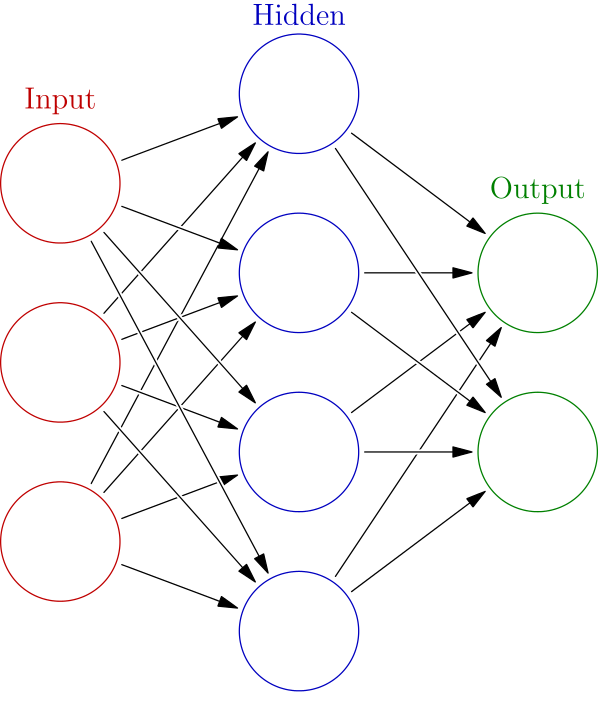
\includegraphics[width=.3\textwidth]{nn}
	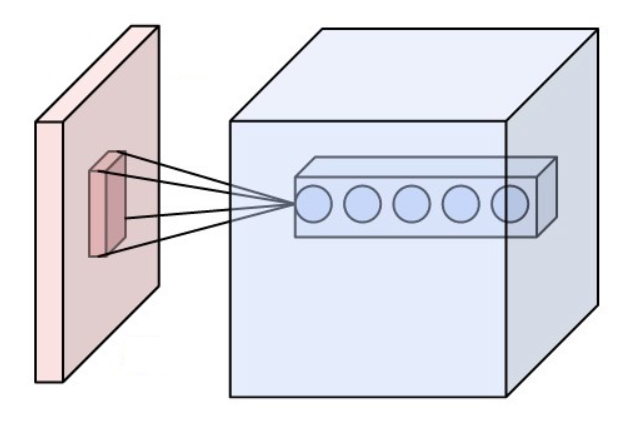
\includegraphics[width=.5\textwidth]{Conv_layer}
	\caption{Left: a very simple neural network with 3-dimensional input (red),  one hidden layer with 4 hidden units (blue),  and 2-dimensional output (green). Right: A pictorial representation of a convolutional layer of a neural network.}
\end{figure}
A \textbf{neural network} is a network of \textbf{neurons}, which represent units of computation organized in \textbf{layers}. (see Figure 2). For example, say we have input 3-dimensional input $\vec{x} = [1,2,3] $. Each of those values would be passed to the input neurons in Figure 1. Then, the first set of black arrows moves the input layer to the hidden layers by multiplying them by some weights and summin]g them together. This is equivalent to multiplying the $3 \times 1$ vector $\vec{x}$ by a $5 \times 3$ matrix of weights, $W$. Then a nonlinear function $f$ is applied elementwise to the 5 dimensional vector $W\vec{x}$. This nonlinear function increases the complexity of the space the neural network can explore, and is usually $f(x) = \tanh(x)$. This process is repeated with the output layer to achieve a $2\times 1$ output vector. In total, the computational process of the neural network can be captured by the equation
$$\vec{output} = f(W^2(f(W^1(\vec{input}))))$$
where $\vec{input}$ is the $3 \times 1$ input data, $W^1$ is the $5 \times 3$ weight matrix for the first layer, $W^2$ is the $2 \times 5$ weight matrix for the second layer, $f$ is an elementwise nonlinear function, and $\vec{output}$ is the $2\times 1$ output vector. The \textbf{activation of a layer}, $F^\ell$ is the intermediary result of running a given input through the network. For example, the activation of the first layer $F^1$ is 
$$F^1= f(W^1(\vec{input}))$$
A \textbf{convolutional neural network} is a neural network is at least one convolutional layer. This neural architecture is inspired by the organization of the human visual cortex, which small regions of neurons are aggregated into a single value. A convolutional layer is a layer that takes a small window of the input data and computes a single value for that region. For example, a \textbf{max pooling} convolutional layer simply computes the maximum value found for a given window (see Figure 2).

Through many layers and complex nonlinearities, a neural network with only a single hidden layer can approximate any function \cite{hornik1991approximation} with sufficient weights. But how are these weight matrices $W^i$ constructed?  This requires \textbf{training} the neural network to configure these weight matrices. In general, this is achieved by feeding it labeled data, $(x,y)$ (with $x_i \in \mathbb{R}^3$ and $y_i \in \mathbb{R}^2$ for our example) and initializing the weights as random. Then, for each observation $x_i$, a prediction $\hat{y}$ is computed by running $x_i$ through the network:
$$\hat{y} = f(W^2(f(W^1(x_i))))$$
Then the error in the network can be computed as the difference between the prediction and the actual output:
$$E(x_i) = (\hat{y} - \hat{y})^2$$
The weights can then be updated by descending the gradient of the error using \textbf{backpropagation}.  A review of the backpropagation algorithm is beyond the scope of this paper, but for a full overview, see \cite{rumelhart1988learning}.

For the purposes of image processing, the input data is raw images $x \in \mathbb{R}^{1000 \times 1000 \times 3}$ assuming they are 1000 pixels by 1000 pixels and are colored. The output $y$ used to trained the network is often labels corresponding to what the image is of, such as: $$y \in \{\text{elephant}, \text{doughut}, \cdots, \text{child},\text{apple}  \}$$
A well documented phenomenon of applying DCNNs to image processing is that lower level layers correspond to pixel or edge level information, and as you look at higher level layers, you get more high order structure. As information passes from the input image pixels to the output classifier, the ``scale'' of that projection increases. For example, layers towards the input correspond to local pixelated regions, edges and neighboring contours. Layers towards the output correspond to global structure, groups of aggregated edges, etc.  The work presented in this paper takes advantage of this important fact.  We will refer to this phenomenon as the visual hierarchy phenomenon (VHP).
\section{Matrix factorization}

Another famous approach for finding the low-rank approximation of a matrix $X$ is  matrix factorization, which aims to find an $A$ and $S$ such that $X \approx AS$ as shown in Figure \ref{nnmf}. Typically, for a input matrix $X \in \mathbb{R}^{n \times m}$ the size of the inner dimension, $k$, is specified ahead of time (such that $A\in \mathbb{R}^{n \times k}$ and $S\in \mathbb{R}^{k \times m})$. Since $k$ is chosen such that $k < \min(m,n)$ we have the was $\operatorname{rank}(AS) = k$, which gives us our low-rank approximation of $S$.

As discussed further in Section \ref{image}, the constraints imposed upon $A$ and $S$ result in different interpretations of the result. For example, constraining the columns of $S$ to be a unary vectors, where one element is equal to one and the other elements are zero, results in the Vector Quantization. Or constraining the columns of $A$ to be orthonormal and the rows of $S$ to be orthogonal to each results in Principal Component Analysis. 

In this thesis, I will focus on a third class of constraints, whereby $A$ and $S$ must be non-negative matrices. This constraint is shown to yield a parts-based approach, which is consistent with a ``topic model'' notion \cite{lee1999learning}." What results is a family of algorithms dubbed \textit{non-negative factorization} or NNMF.

 NNMF was first employed by Paatero and Tapper \cite{paatero1994positive} but was made popular by Lee and Seung \cite{lee1999learning}.
\begin{figure}[h]
	\label{nnmf}
	\centering
	\begin{blockmatrixtabular}
		\valignbox{\fblockmatrix[1.0,0.8,0.8]{1.2in}{0.8in}{$X$}}&
		\valignbox{\mblockmatrix                    {0.15in}{0.8in}{$\approx$}}&
		\valignbox{\fblockmatrix       [0.8,1.0,0.8]{0.6in}{0.8in}{$A$}}&
		\valignbox{\mblockmatrix                    {0.15in}{0.6in}{$\times$}}&
		\valignbox{\fblockmatrix       [0.8,0.8,1.0]{1.2in}{0.6in}{$S$}}&
	\end{blockmatrixtabular}
	\caption{A visual representation of the non-negative matrix factorization}
\end{figure}

The problem of finding such a factorization can be formulated as finding a non-negative $A$ and $S$ that minimize the error 
\begin{align}F = ||X-AS||^2
\end{align}
While this optimization problem is not convex in both $A$ and $S$, it is convex in one of them. So for a given, fixed $S$, we can find the optimal $A$ by setting the gradient equal to zero. Since $||X-AS||^2 = \langle X-AS, X-AS \rangle= X^TX - 2X^TAS + (AS)^T(AS)$ we have
\begin{align*}
\frac{\partial F }{\partial A} ( X^TX - 2X^TAS + (AS)^T(AS)) = 0\\
\text{implies }S^TAS = 2X^TS
\end{align*}
which is to say $\frac{X^TS}{S^TAS}=1$ at the optimal $A$. This equality gives us the below multiplicative update algorithm. 

\begin{algorithm}[H]
	\KwIn{k=0; Initialize $A^0, S^0$}
	\Repeat{Stopping condition}{
		\begin{align*}
		A^{k+1} &= A^k \circ \frac{XS^k}{A^k(S^k)^TA^k}\\
		S^{k+1} &= S^k \circ \frac{XA^{k+1}}{S^k(A^{k+1})^TA^{k+1}}\\
		k &= k+1
		\end{align*} 
	}
	\caption{Multiplicative Update}
\end{algorithm}

This optimization scheme naturally leads to a convex optimization function, so the above algorithm can simply be iteratively applied (until for given $T$ we have $k>T$ or for a given $\epsilon>0$ we have $||X-AS||^2 \leq \epsilon$).
\begin{theorem}
	The Euclidean distance $||X-AS||^2$ is non-increasing under the updating rules of Algorithm 1.
\end{theorem}

A key benefit of non-negative matrix factorization is that its results are very interpretatable. For a given factorization $X \approx AS$, we can think of the $k$ rows of $S$ as a basis $(b_1,b2_,\cdots,b_k)$ for the rows of $X$. Under this interpretation, the row of $A$ give us the linear combination used to form the corresponding row in $X:$
$$X_{i,} = \sum_{j= 1}^k A_{i,j} \times S_{j,}$$
This interpretation is directly applicable to the notion of ``geons as topics'' put forward in Section \ref{interp}. In this thesis, we will focus on NNMF as the central algorithm and we will explore how NNMF can be used to build a theory of visual perception.

\end{chapter}
\begin{chapter}{Types of Data}
	We have defined several algorithmic approaches for the automated understanding of any real valued matrices. In this chapter, we explore how important types of media and data can be represented as real valued matrices. Each section will focus on NNMF as the lens for analysis, and will describe how NNMF can be interpreted in each domain. 
\section{Image}
\label{image}

Because visual object recognition is the foundation of many of the cognitive theories discussed here, it makes sense to think about representing images as data. Because of how computers and digital cameras represent images, they are perhaps the most well suited for representation as data. For gray scale, an image is just a $w \times h$ matrix, where $w$ is the width of the image and $h$ is the height of the matrix. For color, an image is a triple $\{R,B,G\}$ where $R,B,G \in \mathbb{R}^{w \times h}$ correspond to red, blue and green intensities in the image, respectively.
\begin{figure}[h]
	\label{fig:face}
	\centering
	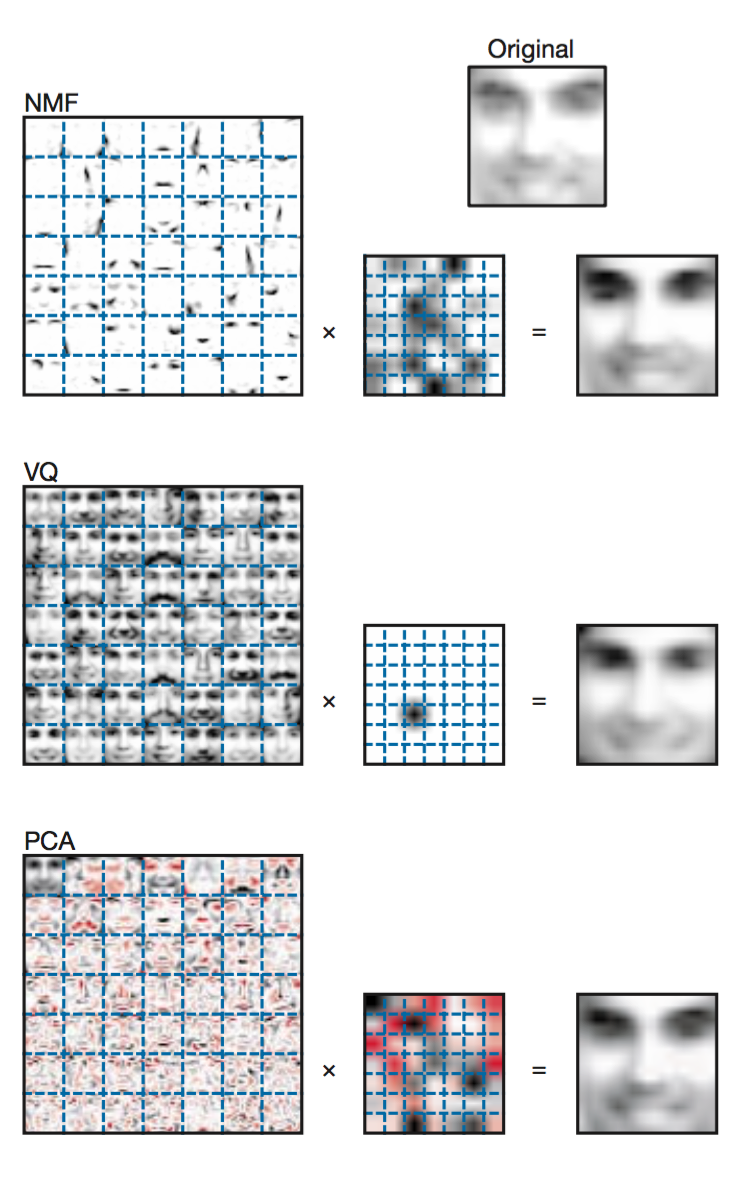
\includegraphics[width=6.2cm]{image}
	\caption{A comparison of the basis vectors learned for NMF, VQ and PCA. Adapted from \cite{lee1999learning}}
\end{figure}
The canonical demonstration of NNMF's ability to learn a parts-based representation utilizes a dataset of faces, $X$, with a row corresponding to a given image and the columns corresponding to a flattened vector representation of the matrix. Lee and Seung compare the NNMF factorization of this corpus with vector quantification (VQ) and principal component analysis (PCA). Indeed all three methods attempt to factorize $X$ into two matrices $A$ and $S$: the only difference is the constraints imposed on $A$ and $S$. As we have seen, NNMF does not allow nonnegative entries in either $A$ and $S$. For VQ, each column of $S$ is constrained to be a unary vector. And finally PCA contrains the colums of $A$ to be orthonormal and rows of $S$ to be orthogonal to each other \cite{lee1999learning}.

As can be seen in Figure \ref{fig:face}, the bases each approach learns is radically different. VQ learns a basis of prototypes, where each basis itself is an entire face, and each row of $X$ is a linear combination (i.e. addition and subtraction) of these protofaces. Alternatively, PCA learns a basis of `eigenfaces,' which correspond to ``distored'' versions of complete faces \cite{turk1991eigenfaces}. Instead of learning a``holistic'' representation of the faces like VQ and PCA, NMF learns a parts-based model, where the rows of $S$ correspond to discrete components of a face. 

\section{Sound}
Despite not being as discrete as images or graphs, sound also can be represented in a high structured way. There have been many approaches to do so. Perhaps the most success is the Deep Speech models, which feed speech snippets into a RNN paired with a language model for real time dictation \cite{amodei2015deep,hannun2014deep}. These Deep Speech systems represent sound as follows. An utterance $x$ is a time series of length $T$	sliced into time intervals $t$. For each time interval, the utterence is represented as a vector of audio features, $\vec{x_t}$. Hannun et al, in their famous Deep Speech neural model, use spectrograms as features, such that $\vec{x_{t,p}}$ is the power of the $p$th frequency bin the the audio frame at time $t$ \cite{hannun2014deep}.

Another approach is to take the modulus of a given signal's the STFT as treat that spectrogram  $X$ as a matrix to be factorized \cite{kawamoto2000estimation,krause2015non}. NNMF is particularly useful in this domain because the source components (the results of the factorization) are also interpreted as spectrograms, which must have non-negative entries. 
\section{Graph}
Since a network of edges and vertices $G=(V,E)$ can be represented as an \textit{adjacency matrix} $A \in \{0,1\}^{|V| \times |V|}$ with $A_{i,j} = 1$ if $(i,j) \in E$ and $A_{i,j}=0$ otherwise, graphs are another domain well suited for low dimensional representations. \footnote{For now, we will work with unweighted, undirected graphs, although these results generalize to other types of graphs as well.} Factorizing this adjacency matrix is equivalent to clustering the graph, which is a central problem to graph theory \cite{ho2008nonnegative}.
A given clustering $C = \{C_1, C_2, \cdots, C_k\}$ of a graph is a partition of the vertices and can be evaluated based on its \textit{connectivity}:
$$\text{connectivity}(G,C) = \frac{\#\{(i,j)\in E | (i,j) \in C\} + \#\{(i,j)\not\in E | (i,j) \not\in C\}}{|V|^2}$$
The clustering $C$ can be formulated as a membership matrix $M \in \{0,1\}^{n \times k}$ with $M_{ir}=1$ if $i \in C_r$ and $X_{ir}$ if $i \not\in C_r$. Thus, the connectivity of $G$ under $C$ as defined above can be rewritten:
\begin{align*}\text{connectivity}(G,C)  &= 1-\frac{\sum_{i,j} \left(A_ij - \sum_{r=1}^k X_{ir}X_{jr}\right)^2}{|V|^2}\\
&=1-\frac{||A-XX^T||^2_F}{|V|^2}
\end{align*}
Thus finding a clustering $C$ that maximizes the connectivity is equivalent to the minimization problem 
$$\min_{X \in \{0,1\}^{n\times k}} ||A-XX^T||^2_F$$
However, finding one such $X$ is NP-Complete \cite{vavasis2009complexity}. So we can relax the constraints to try to solve an easier problem we are more used to 
$$\min_{X \in \mathbb{R}_{+}^{n\times k}} ||A-XX^T||^2_F$$
which just the standard optimization for non-negative matrix factorization for the symmetric case. Since the $X$ we are solving for in this case is no longer binary, but rather contains reals, it is considered a \textit{weak membership matrix}. That is, the larger $X_{i,j}$, the stronger membership of vertex $i$ in cluster $j$. 
\section{Natural Language}
With the vast amount of digital text being generated across the internet, methods for understanding and processing corpora of human language become necessary. Across mathematics and computer science, many techniques have been put forward that allow one to understand a body of text far too large to read herself. A successful method in this domain is \emph{topic modelling}, whereby semantically cohesive subgroups of words can be identified. In particular, let $\mathcal{C} = \{d_1,d_2,\cdots, d_n\}$ be a collection of documents with a vocabulary $\mathcal{V}$. A \emph{topic}  $t_i$ is a vector over the words in the vocabulary that represents a coherent high level notion in the corpus:
$$t_i = \{v^i_1, v^i_2, \cdots, v_m^i\}$$
where $m$ is the size of the vocabulary. Topic modelling offers a powerful tool for understanding large amounts of text because they can discover latent semantic structure within text. 

There are two primary techniques for learning these topics $t_i$. The first is LDA, a generative Bayesian statistical model which views each document $d_j$ as a mixture of various topics.
The second is non-negative matrix factorization, which aims to factor the document/word matrix into a document/topic and a topic/word matrix \cite{lee1999learning}. The focus of this thesis will be NNMF, because of its relation to linear algebra, and its deep visual and conceptual intuition. 

Given our $n$ documents with vocabulary $\mathcal{V}$ of size $m$, we construct a matrix $X \in \mathbb{R}^{n\times m}$ where $X_{i,j}$ is the number of occurences of word $j$ in document $i$. For a given inner dimension $k$, we seek to factor $X$ into two matrices $A$ and $S$ such that
$$X \approx AS$$
where $A \in \mathbb{R}^{n\times k}$ is the document/topic matrix and  $S \in \mathbb{R}^{k\times m}$ is the topic/word matrix. When we impose that $A$ and $S$ must be non-negative, a strong intuition emerges. In particular, the $(i,j)$th entry of $A$ corresponds to the proportion of topic $j$ in document $i$ and the $(i,j)$th entry of $S$ corresponds to the relevance of word $j$ in topic $i$.
\end{chapter}

\begin{chapter}{Semi-Supervised NNMF}
	The methods above are unsupervised, which means the algorithms are designed to reveal latent structure within the unlabeled data. Many times however, data is accompanied with labels and the new algorithmic objective is to assign new unobserved data into appropriate labels. In the semi-supervised case, when only some of the data is labeled, the objective is similar to the unsupervised case. However, the known class labels can be incorporated into the model to improve classification performance \cite{lee2010semi}. In this section, we will explore an extension of NNMF where some of the class labels are known, and this information is used to enhance the performance of the NNMF. This \emph{semi-supervised} NNMF  learns a one-versus all separating hyperplane for the observations \cite{lee2010semi}.
	\section{Approach}
	In many cases, in addition to  $X \in \mathbb{R}^{n\times m}$ we also have a label matrix $Y \in \mathbb{R}^{n\times k}$, where $k$ is the number of classes and $Y_{i,j}$ is 1 if document $i$ is in class $j$ and 0 otherwise. 
	Given $B \in \mathbb{R}^{k \times r}$, a basis matrix for $Y$, and $L \in \mathbb{R}^{k \times n}$, a weight matrix to handle missing labels, then the energy function for SSNMF is as follows
	$$E - ||(X-AS)||^2 + \lambda ||L \circ (Y-BS)||^2$$
	where $\lambda$ is a tradeoff parameter that governs the importance of the supervised term.
	
	In the same vein of Algorithm 1, this energy function yields a convex optimization problem solved by the following algorithm. 
	
	\begin{algorithm}[H]
		\KwIn{k=0; Initialize $A^0, S^0, B^0$}
		\Repeat{Stopping condition}{
			\begin{align*}
			A^{k+1} &= A^k \circ \frac{XS^k}{A^k(S^k)^TS^k}\\
			B^{k+1} &= B^k \circ \frac{(L \circ Y )S^k}{(L \circ B(S^k)^T)S^k}\\
			S^{k+1} &= S^k \circ \frac{(A^{k+1})^TX + \lambda B^T (L \circ Y)}{(A^{k+1})^TAS + \lambda B^T (L \circ BS)}\\
			k &= k+1
			\end{align*} 
		}
		\caption{Multiplicative Update for Semi-Supervised NNMF}
	\end{algorithm}
	\section{Visualization}
\begin{center}
	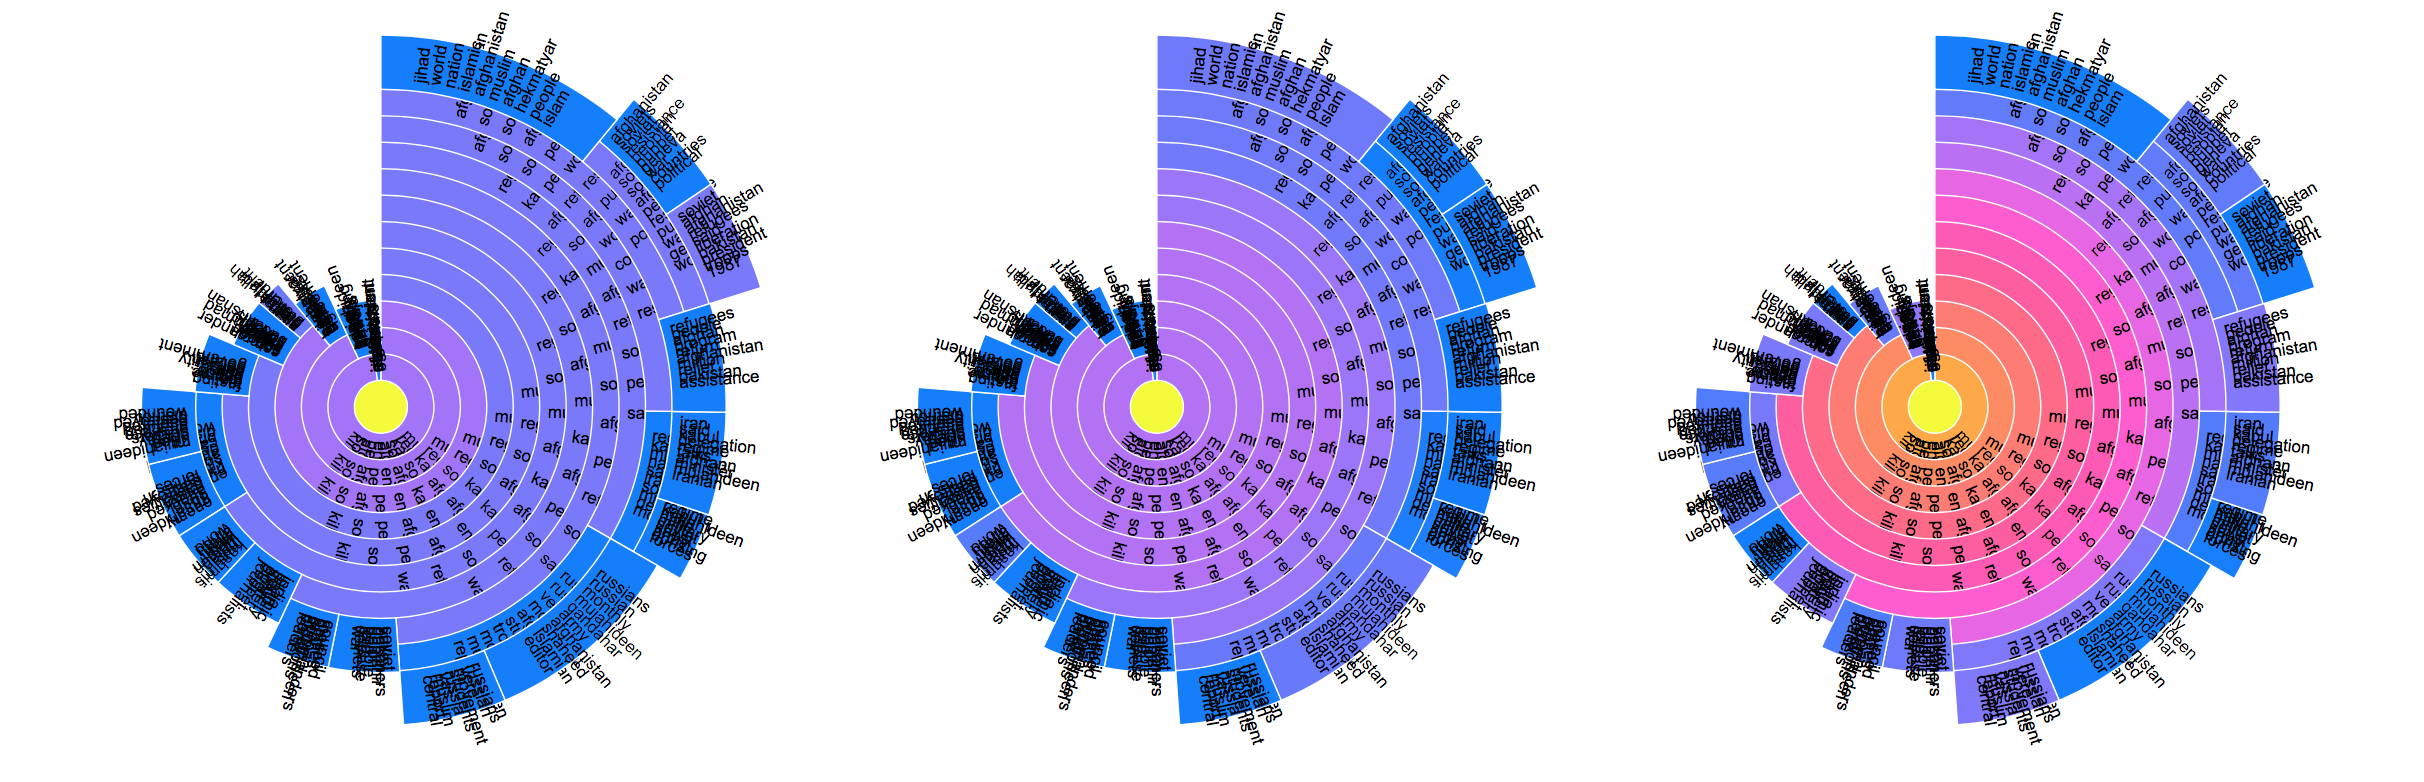
\includegraphics[width=7	in]{semi-viz}
\end{center}
\end{chapter}
\begin{chapter}{Hierarchical Representation}
Many times, the data we wish to represent exhibits hierarchical structure. One such example is with the topics found in text data. Since topics correspond to semantic ideas, it makes sense that they would be organized in hierarchicaly. For example, in the 20 News Group data set, there are two separate topics for the Cincinnati Reds and Toronto Blue Jays, two baseball teams. Thus one could think about a supertopic, baseball, that branches into the two topics the standard NNMF finds.
\section{Approach}
For a given document matrix $V$, we use the python library \texttt{scikitlearn} to decompose $V$ into document/topic matrix $W$ and topic/word matrix $H$ such that $$V \approx WH.$$ The  \texttt{scikitlearn} implementation uses alternating gradient descent with the following objective function to generate optimal guesses for $W$ and $H$.
$$c(H,W) = \tfrac{1}{2} ||X-WH||_{fro}^2 + \alpha \lambda ||W||_1 + \alpha \lambda ||H||_1 + \tfrac{1}{2} \alpha (1-\lambda) ||W||^2_{fro} + \tfrac{1}{2} \alpha (1-\lambda) ||H||^2_{fro}  $$
where $||\cdot||_{fro}$ is the Frobenius norm, $||\cdot||_{1}$ is the L1 norm, $\lambda$ is the L1 ratio and $\alpha$ is a free parameter. 

From the $N$ topics $t_n$ for $n \in \{1\cdots N\}$\footnote{observe that $t_n$ is simply the $n$th row of $H$}, we populate an adjacency matrix $A$ where $$A_{i,j} = \frac{T_i \cdot T_j}{||T_i|| \ ||T_j||}$$ is the cosine similarity between topics $i$ and $j$. We then define a \emph{threshold vector} $\sigma$ by sorting all the elements of $A$. $$\sigma = \{\sigma_1, \sigma_2, \cdots \sigma_{N^2} \mid0 \leq \sigma_{i} \leq \sigma_j \leq 1 \forall i \leq j\text{ and }\sigma_k \in A\}$$
We then create an array of graphs $A^{(k)}$ thresholded using the values of $\sigma$, such that  \[
A^{(k)}_{i,j} =
\begin{cases}
1 & \text{if } A_{i,j} >\sigma_k\\
0 & \text{otherwise.}
\end{cases}
\]
Observe that $A^{(1)}$ is the fully connected graph and $A^{(N^2)}$ is the completely disconnnected graph.
By looking at the connected components  of a given graph,
$$c(A^{(j)})=\{c^j_1, c^j_2,\cdots,c^j_i,\cdots,c^j_N\}$$
where $c_i =k$ means that the $i$th vertex is in the $k$th order component, we can formulate a tree structure (see Figure 1).
\begin{figure}
	\centering
	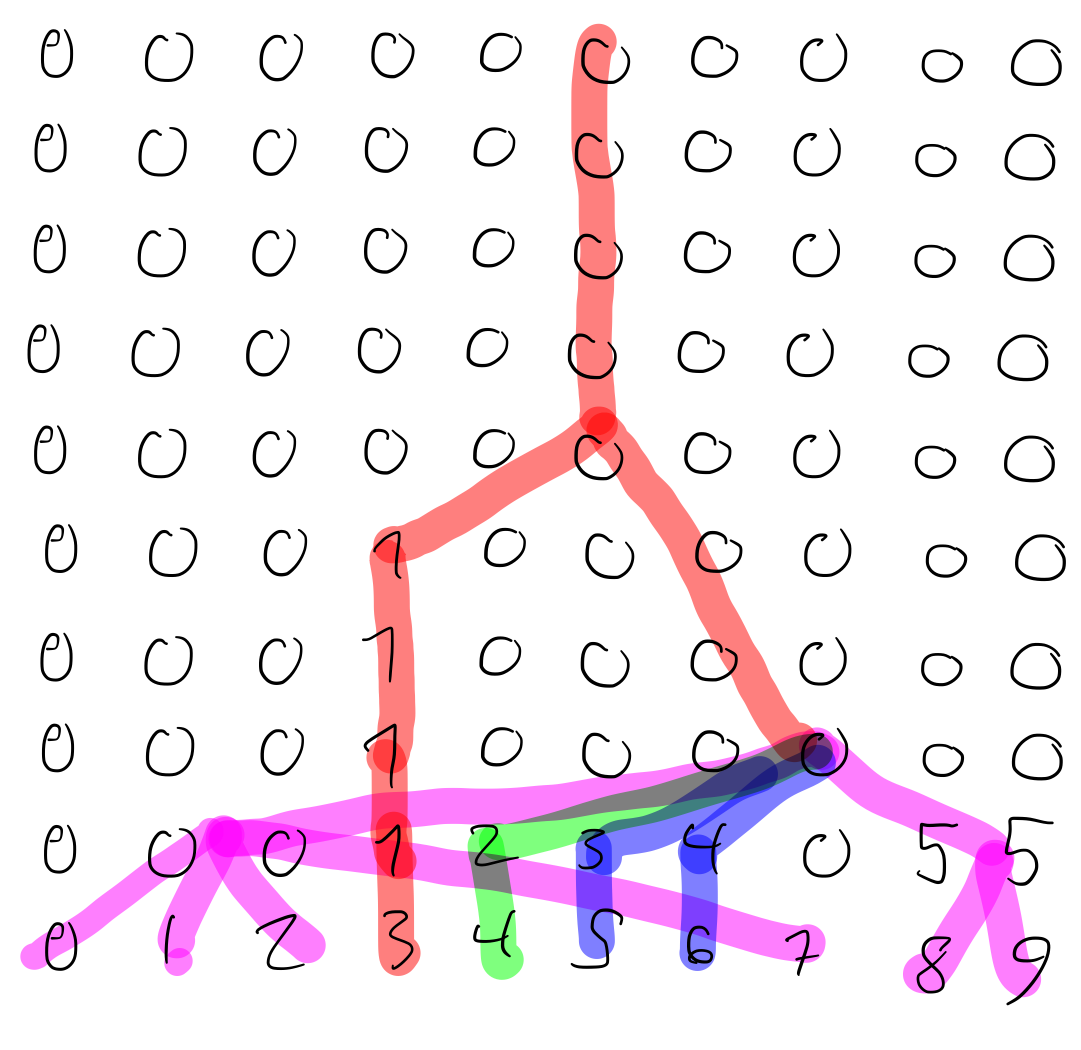
\includegraphics[width=.5\textwidth]{tree}
	\caption{How the tree structure is formed for the connected componenet vectors}
\end{figure}
For example, say $N=8$ and we have
\begin{align*}
c(A^{(j)})=\{0, 0, 0 ,0, 1 ,1 ,1, 1\}\\
c(A^{(j+1)})=\{0, 0, 0 ,0, 1 ,1 ,2, 2\}
\end{align*}
This means that $A^{(j)}$ has two connected components, ordered 0 (with vertices 1,2,3,4) and 1 (with vertices 5,6,7,8) and that $A^{(j+1)}$ has three connected components, ordered 0 (with vertices 1,2,3,4), 1 (with vertices 5 and 6) and 2 (with vertices 7 and 8).  Thus there is a branch from the connect component 1 in $A^{(j)}$ to the connected componenets 1 and 2 in $A^{(j+1)}$. By greedily repeating this iterative algorithm starting with $A^{(1)}$ \footnote{which has by definition only a single connected component and so $c(A^{(1)})=\{0, \cdots, 0\}$} as the root, we produce the tree of topics. Observe that at this stage, all the leaf nodes correspond to actual topics $t_n$. We formulate the topic vectors for the parent nodes by additive percolating up the tree. That is, for a given parent topic $\tau$ with children $\tau_1, \cdots, \tau_k$ we simply have 
$$\tau =\sum_i \tau_i $$
\section{Visualization}
\begin{figure}
	\centering
	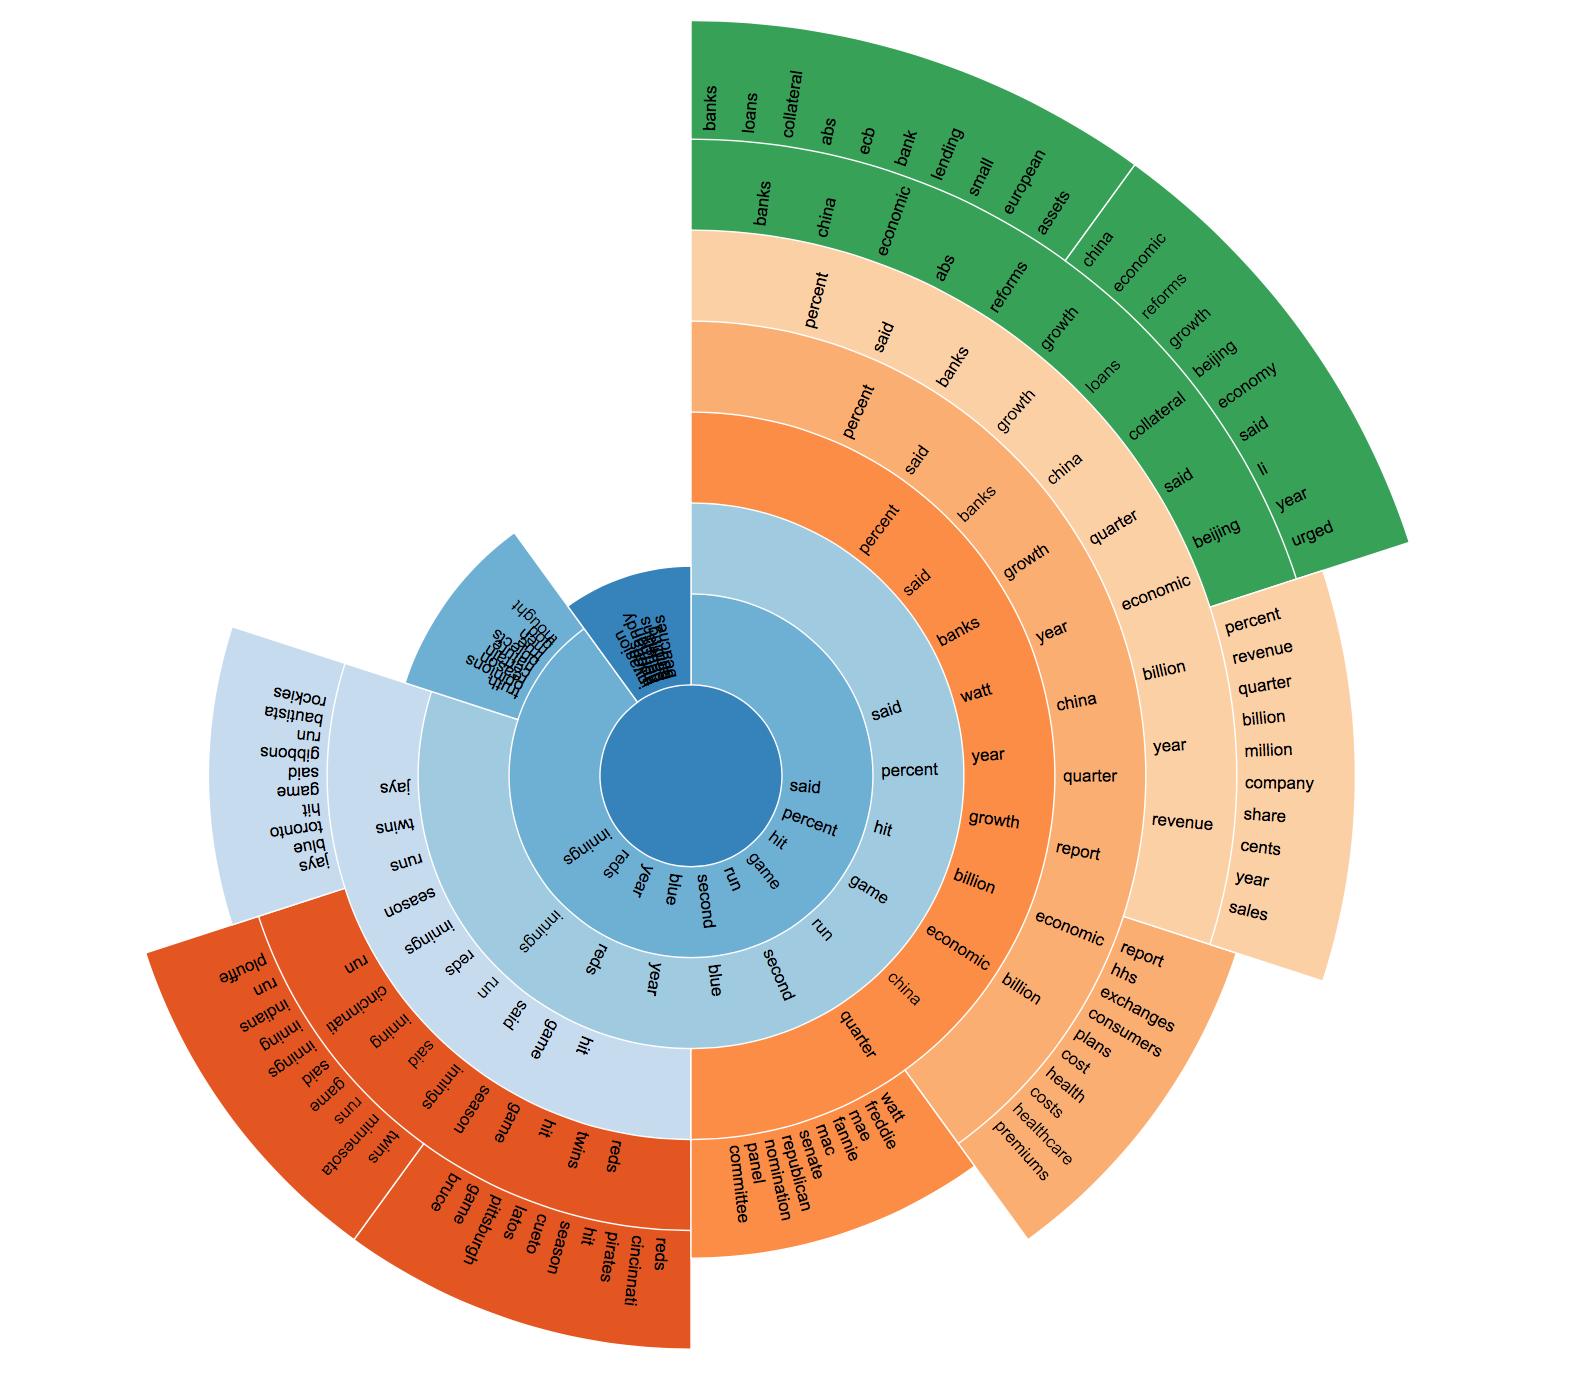
\includegraphics[width=.48\textwidth]{img}
	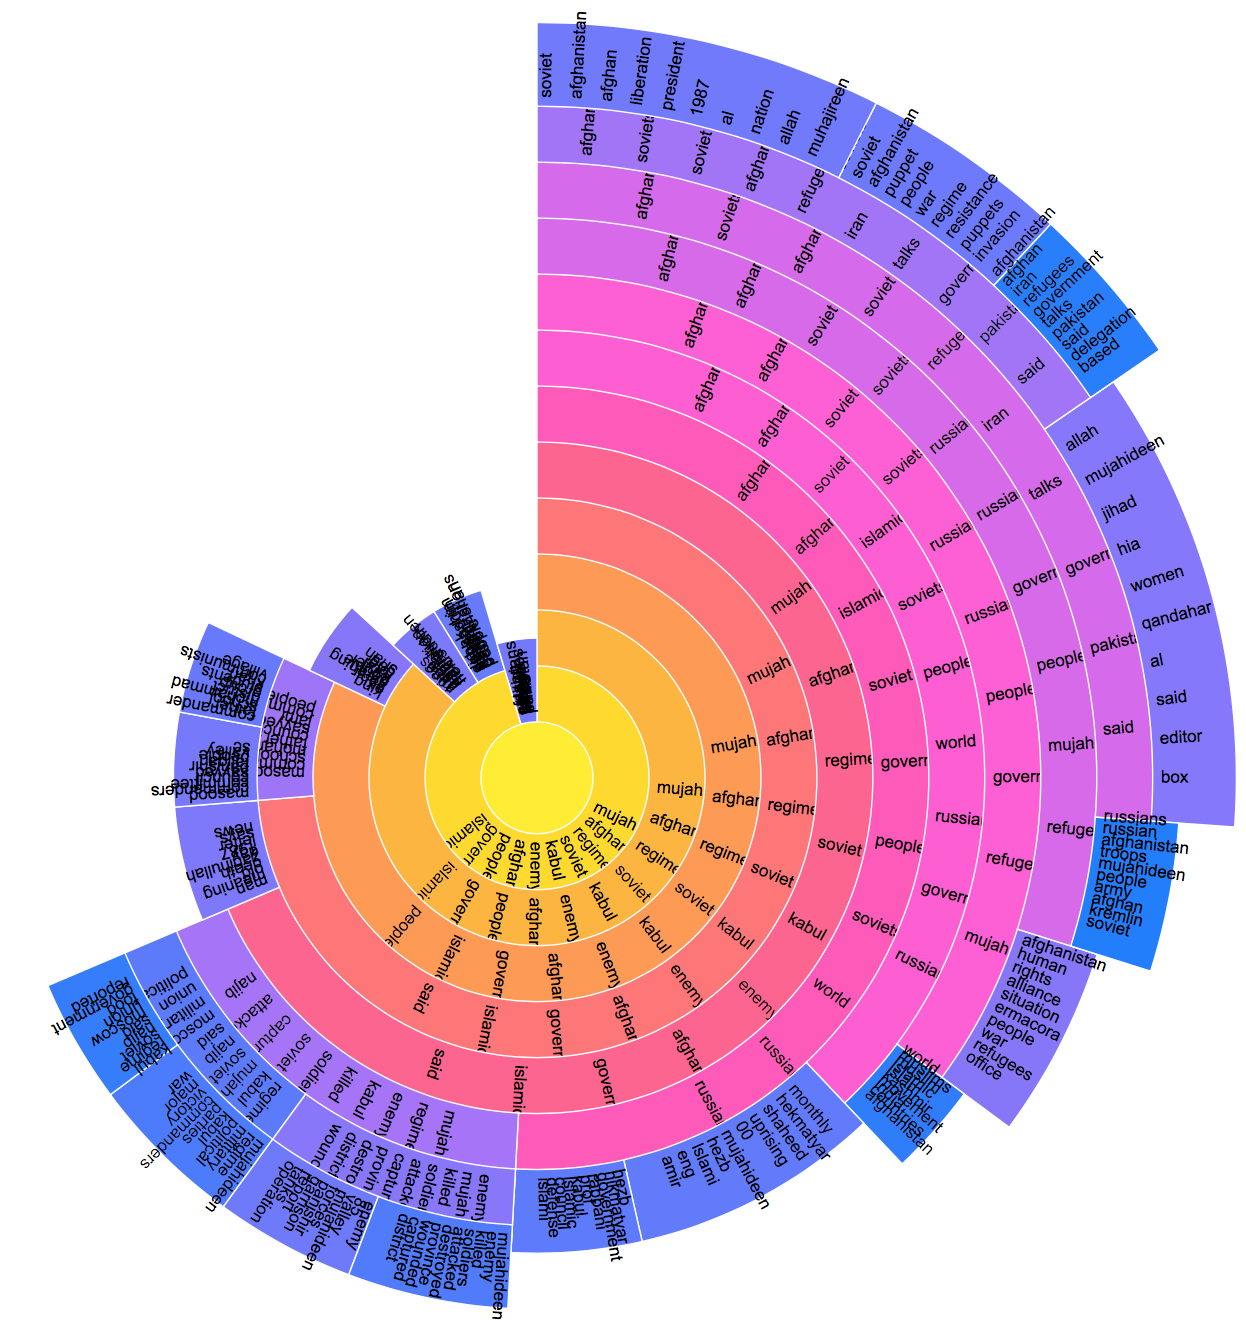
\includegraphics[width=.48\textwidth]{img2}
	\caption{Left: Visualization of hierarchical topics in standard NMF; Right: Visualization of hierarchical topics in  SSNMF; }
\end{figure}
I use the d3.js Sunburst implementation to visualize the hierarchical topic model. Arcs at the same level represent discrete topics. A topic on an inner layer that encompasses multiple outer topics represent a super-topic. For example, in Figure 3, the two outer green topics that represent European banking and Chinese banking representatively (with top words$$ \{\text{banks, loans, collateral, abs, ecb bank, lending, small, european, asset}\} $$and $$\{\text{china, economic, reforms, growth, beijing, economy, said, li, year, urged}\}) $$merge into the inner super topic with top words$$ \{\text{banks, china, economic, abs, reforms, growth, loans, collateral, said, beijing}\}.$$

The visualization is responsive, dynamic and available at \\ \texttt{http://www1.cmc.edu/pages/faculty/BHunter/ziv.html}

Next, I extended this visualization to the Semi-Supervised domain using the Afghan Dataset. Here each document has associated with it a class $C\in \{1,\cdots,k\}$ which in this case $k=3$. Recall that the matrix $B \in \mathbb{R}^{k \times r}$ in the semi-supervised NMF model is multiplied by $S$ to obtain an approximation for $Y$, the label matrix. Thus the $i,j$th entry of $B$ can be interpreted in the weighted importance of topic $i$ in predicting class $j$. Thus I sum over the columns of $B$ to capture how important topic $i$ is predicting classes in general. After normalizing, we get a color value $c_i$ for topic $i$, such that
$$c_i = \sum_j B_{i,j} /  \sum_{i,j} B_{i,j}$$
where $c_i=1$ corresponds to yellow and $c_i=0$ corresponds to blue (see Figure 3 right)
\end{chapter}

\begin{chapter}{Deep Models}
\section{Approach}
Semi-Supervised NNMF as discussed above can be thought of as representing $A$ in a low dimensional representation as $S$. In this framework, $A$ is the function that maps the low dimensional representation to the original high dimensional representation. However, as the data becomes increasingly complex, it may have many hierarchy of attributes, each of which requires its own mappings. With the motivation in mind, Trigeorgis et al put forward the notion of a Demi-Semi NNMF \cite{trigeorgis2014deep}.
$$X \approx A_1A_2 \cdots A_m S_m$$
This representation of the data can be achieved by recursively factorizing the low-dimensional representation at each level \cite{trigeorgis2014deep}.
\begin{align*}
S_{m-1} = A_mS_m\\
\vdots \\
S_2  \approx A_3 \cdots A_m  S_m\\
S_1  \approx A_2 \cdots A_m  S_m
\end{align*}

We then consider the algorithms and notions in the domain of Deep Semi NMF as a model for Hierarchical NMF \cite{ deepNonNeg, trigeorgis2014deep} 
\section{Deep Neural Models}
\section{Visualization}
	\end{chapter}
\begin{chapter}{Discussion}
	\end{chapter}


\bibliographystyle{plain}

\bibliography{myBib}
\end{document}